% =====================================================================
%  CENG 252 -- Practice Midterm 2 (Lectures 6--10)
%  Compile with pdflatex.  Solutions: Practice_Midterm2_Solutions.tex
% =====================================================================
\documentclass[11pt]{article}
\usepackage[margin=2.2cm,headheight=14pt]{geometry}
\usepackage{amsmath,amssymb}
\usepackage[version=4]{mhchem}
\usepackage{tikz}
\usepackage{pgfplots}
\pgfplotsset{compat=1.17}
\usepackage[most]{tcolorbox}
\usepackage{booktabs,array}
\usepackage{enumitem}
\usepackage{fancyhdr}
\usepackage{lastpage}
\usepackage{lmodern}
\usepackage[T1]{fontenc}
\usepackage{multicol}

\setlength{\parindent}{0pt}
\setlength{\parskip}{4pt}
\pagestyle{fancy}
\fancyhf{}
\lhead{\small CENG 252 \textbullet\ Practice Midterm 2}
\rhead{\small Name: \underline{\hspace{5cm}}}
\cfoot{\small Page \thepage\ of \pageref{LastPage}}

\newcommand{\AS}[1]{\mathrm{#1\!\cdot\!S}}
\newcommand{\problem}[2]{\section*{Problem #1: #2}}
\newcommand{\pts}[1]{\hfill\textbf{[#1 pts]}}
\newcommand{\workspace}[1]{\par\vspace{#1}}

\begin{document}

\begin{center}
{\LARGE\bfseries CENG 252: Chemical Reaction Engineering}\\[6pt]
{\Large Practice Midterm 2 (Lectures 6--10)}\\[4pt]
Time: 1 hour 20 minutes \quad\textbullet\quad Total: 100 points
\end{center}

\begin{tcolorbox}[colback=white,colframe=black!70,title=\textbf{Instructions},fonttitle=\bfseries]
\begin{itemize}[itemsep=2pt]
\item Closed book, closed notes, no cheat sheet. A formula sheet is provided on the last page. Only a simple scientific calculator.
\item \textbf{Show all work.} For mechanisms: write every elementary step's rate law, state which species each $k$ refers to,
apply the PSSH or the equilibrium of the fast steps, and write the conservation (enzyme or site) balance \emph{before} simplifying.
Partial credit is given for a correct setup.
\item State every assumption. Box your final answers and include units.
\item Budget your time: about 0.8 minutes per point (16 minutes for a 20-point problem).
\end{itemize}
\end{tcolorbox}

\begin{center}
\renewcommand{\arraystretch}{1.35}
\begin{tabular}{clcc}
\toprule
Problem & Topic & Points & Score\\
\midrule
1 & Short answers (PSSH, L--H, inhibition, deactivation) & 15 & \\
2 & Active intermediates and the PSSH: ozone decomposition & 20 & \\
3 & Enzyme kinetics, inhibition and a batch bioreactor & 25 & \\
4 & Heterogeneous catalysis: mechanism, data, reactor and deactivation & 40 & \\
\midrule
 & \textbf{Total} & \textbf{100} & \\
\bottomrule
\end{tabular}
\end{center}

\textbf{Constants:} $R=8.314$ J/(mol$\cdot$K) $=1.987$ cal/(mol$\cdot$K) $=0.08206$ dm$^3\cdot$atm/(mol$\cdot$K).

% =====================================================================
\newpage
\problem{1}{Short answers}\pts{15}

\textbf{(a) [3]} The termination step of a free-radical chain is \ce{2CH3^{.} ->[k_5] C2H6}, with $k_5$ defined with
respect to C$_2$H$_6$, so $r_{5,\mathrm{C_2H_6}}=k_5C_{\mathrm{CH_3\bullet}}^2$. Write the term that this step contributes
to the PSSH balance for CH$_3\bullet$. Explain the factor.
\workspace{3.2cm}

\textbf{(b) [3]} A catalytic hydrogenation \ce{A + H2 -> B} has the measured rate law
\[
-r_A'=\frac{k\,P_A\,P_{\mathrm{H_2}}^{1/2}}{\left(1+K_AP_A+\sqrt{K_{\mathrm{H}}P_{\mathrm{H_2}}}\right)^2}.
\]
Give three conclusions about the mechanism that you can read directly from this expression.
\workspace{3.6cm}

\textbf{(c) [3]} Two inhibitors each lower the rate of an enzyme reaction. With inhibitor X, the Lineweaver--Burk line keeps
the same intercept but becomes steeper. With inhibitor Y, the line shifts up parallel to the original. Name each
type. For which one can the original $V_{\max}$ still be reached by adding a large excess of substrate? Why?
\workspace{3.6cm}

\newpage
\textbf{(d) [3]} The initial rate of \ce{A -> B} over a solid catalyst was measured against the feed pressure of pure A for three
different catalysts. Match each curve (i), (ii), (iii) to its rate-limiting step (adsorption of A, single-site surface
reaction, or dual-site surface reaction), and give one sentence of justification for each.
\begin{center}
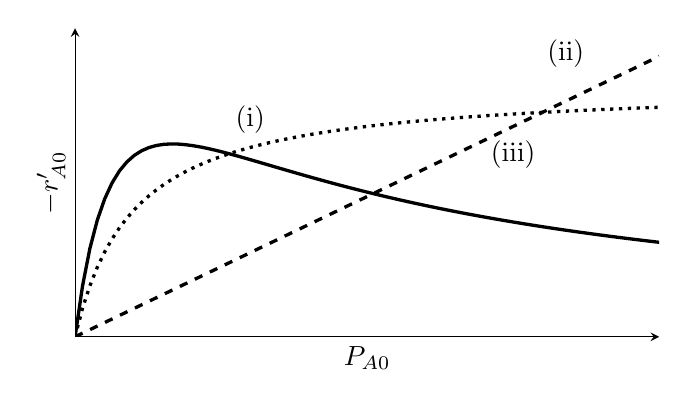
\begin{tikzpicture}
\begin{axis}[width=9cm,height=5.5cm,xmin=0,xmax=10,ymin=0,ymax=2.2,axis lines=left,
  xlabel={$P_{A0}$},ylabel={$-r_{A0}'$},ticks=none]
\addplot[very thick,domain=0:10,samples=80]{6*x/(1+0.6*x)^2*0.55};
\node at (axis cs:3.0,1.55) {(i)};
\addplot[very thick,dashed,domain=0:10]{0.2*x};
\node at (axis cs:8.4,2.02) {(ii)};
\addplot[very thick,dotted,domain=0:10,samples=80]{1.8*x/(1+1.0*x)};
\node at (axis cs:7.5,1.30) {(iii)};
\end{axis}
\end{tikzpicture}
\end{center}
\workspace{2.8cm}

\textbf{(e) [3]} The activity of a reforming catalyst was measured as $a=0.80$ after 10 h and $a=0.50$ after 40 h. Show
whether first-order or second-order decay fits these data. Name the deactivation mechanism that usually gives this order,
and find the time at which $a=0.25$.
\workspace{4cm}

% =====================================================================
\newpage
\problem{2}{Active intermediates: ozone decomposition}\pts{20}

The gas-phase decomposition \ce{2O3 -> 3O2} is believed to go through atomic oxygen, O, as an active intermediate:
\[
\text{(1)}\ \ce{O3 ->[k_1] O2 + O}\qquad
\text{(2)}\ \ce{O2 + O ->[k_2] O3}\qquad
\text{(3)}\ \ce{O + O3 ->[k_3] 2O2}
\]
All rate constants are defined with respect to the species O. Every step is elementary.

\textbf{(a) [8]} Use the PSSH to derive the rate of disappearance of ozone, $-r_{\mathrm{O_3}}$, in terms of measurable
concentrations only.
\workspace{7.5cm}

\textbf{(b) [5]} Experiments carried out in a large excess of O$_2$ give $-r_{\mathrm{O_3}}=k_{\text{obs}}\dfrac{C_{\mathrm{O_3}}^2}{C_{\mathrm{O_2}}}$.
State the condition under which your result reduces to this form, and express $k_{\text{obs}}$ in terms of $k_1,k_2,k_3$.
What rate law do you expect at the very start of a run that begins with pure ozone?
\workspace{5cm}

\newpage
\textbf{(c) [4]} The activation energies of the elementary steps are $E_1=100$ kJ/mol, $E_2=2$ kJ/mol and $E_3=20$ kJ/mol.
Find the apparent activation energy of $k_{\text{obs}}$. By what factor does $k_{\text{obs}}$ increase from 300 K to 310 K?
\workspace{5cm}

\textbf{(d) [3]} At a fixed, moderate O$_2$ concentration, sketch $-r_{\mathrm{O_3}}$ versus $C_{\mathrm{O_3}}$ over a wide range of
$C_{\mathrm{O_3}}$, and label the apparent reaction order in each region. Which elementary step limits the rate at high $C_{\mathrm{O_3}}$?
\workspace{5cm}

% =====================================================================
\newpage
\problem{3}{Enzyme kinetics, inhibition and a batch bioreactor}\pts{25}

An enzyme E converts substrate S to product P by the Michaelis--Menten mechanism
\ce{E + S <=> E.S -> E + P}. The initial rates below were measured at the same total enzyme concentration, first with no
inhibitor and then with an inhibitor I at $C_I=4.0$ mmol/L.

\begin{center}
\renewcommand{\arraystretch}{1.3}
\begin{tabular}{lccccc}
\toprule
$C_S$ (mmol/L) & 1.0 & 2.0 & 5.0 & 10.0 & 20.0\\
\midrule
$-r_S$, no inhibitor (mmol/L/min) & 0.333 & 0.571 & 1.000 & 1.333 & 1.600\\
$-r_S$, with $C_I=4.0$ mmol/L (mmol/L/min) & 0.250 & 0.364 & 0.500 & 0.571 & 0.615\\
\bottomrule
\end{tabular}
\end{center}

\textbf{(a) [7]} In \emph{uncompetitive} inhibition, I binds only to the enzyme--substrate complex:
\ce{E.S + I <=> I.E.S} (inactive), with $K_I=C_{E\cdot S}C_I/C_{I\cdot E\cdot S}$. Starting from the mechanism and the total enzyme
balance, derive $-r_S$ for uncompetitive inhibition and write it in Lineweaver--Burk (reciprocal) form. State what happens to
the slope and the intercept compared with no inhibition.
\workspace{7cm}

\newpage
\textbf{(b) [6]} Using a Lineweaver--Burk analysis of the uninhibited data, find $V_{\max}$ and $K_M$ (with units).
\workspace{6cm}

\textbf{(c) [5]} Analyse the inhibited data the same way. Which type of inhibition is this? Find $K_I$.
\workspace{5.5cm}

\newpage
\textbf{(d) [7]} The same enzyme loading is used in a well-mixed, constant-volume batch reactor with $C_{S0}=20$ mmol/L.
Starting from the mole balance, derive an expression for the time needed to reach conversion $X$, and compute the time for
$X=0.90$ (i) with no inhibitor and (ii) with $C_I=4.0$ mmol/L held constant. Explain in one sentence why the inhibitor has
almost no effect late in the batch, when $C_S$ is small.
\workspace{9cm}

% =====================================================================
\newpage
\problem{4}{Heterogeneous catalysis: from mechanism to reactor}\pts{40}

The gas-phase dehydration of an alcohol A to an olefin B and water W, \ce{A -> B + W}, is carried out over a solid acid
catalyst at 500 K. The proposed mechanism is
\[
\text{(1)}\ \ce{A + S <=> A.S}\qquad
\text{(2)}\ \ce{A.S + S -> B.S + W.S}\qquad
\text{(3)}\ \ce{B.S <=> B + S}\qquad
\text{(4)}\ \ce{W.S <=> W + S}
\]
Step (2) is irreversible. Use adsorption equilibrium constants $K_A$, $K_B$, $K_W$, and $C_t$ for the total site concentration.

\textbf{(a) [8]} Derive the rate law $-r_A'$ assuming the surface reaction (2) is rate-limiting. Show the site balance.
\workspace{7cm}

\textbf{(b) [6]} Derive the rate law assuming instead that the adsorption of A (step 1) is rate-limiting. (Hint: what does
``fast and irreversible'' imply for $C_{\AS{A}}$?) Write the initial rate for each of the two cases, (a) and (b).
\workspace{5.5cm}

\newpage
\textbf{(c) [9]} Initial rates measured with pure A in the feed (no B or W present) are:
\begin{center}
\renewcommand{\arraystretch}{1.3}
\begin{tabular}{lccccc}
\toprule
$P_{A0}$ (atm) & 0.5 & 1.0 & 2.0 & 4.0 & 8.0\\
\midrule
$-r_{A0}'$ (mol/kg cat/s) & 0.160 & 0.222 & 0.250 & 0.222 & 0.160\\
\bottomrule
\end{tabular}
\end{center}
Which of your rate laws, (a) or (b), is consistent with these data? Explain. Using a suitable linearisation, determine the
lumped rate constant $k$ (with units) and $K_A$.
\workspace{8cm}

\newpage
\textbf{(d) [9]} Separate experiments show that B and W are only weakly adsorbed ($K_BP_B,\,K_WP_W\ll1$).
The reaction is run in a fluidised-bed reactor that behaves as a CSTR, isothermal at 500 K with no pressure drop.
Pure A is fed at $F_{A0}=10$ mol/s.
\begin{enumerate}[label=(\roman*),itemsep=2pt]
\item Find the catalyst mass needed for $X=0.50$ when the inlet pressure is $P_0=2$ atm.
\item An engineer suggests that a higher pressure always means a faster rate. At the same $F_{A0}$ and $X=0.50$, what inlet pressure
\emph{minimises} the catalyst mass, and what is that minimum mass? Explain physically why raising the pressure further
does not help.
\end{enumerate}
\workspace{8cm}

\newpage
\textbf{(e) [8]} The reactor is now operated at the optimum from (d)(ii). The catalyst sinters, following second-order decay with
$k_d=0.0125$ h$^{-1}$. The fluidised bed is well mixed, so all of the catalyst has the same age.
\begin{enumerate}[label=(\roman*),itemsep=2pt]
\item Find the activity after 80 h. To what value must $F_{A0}$ be reduced (same $P_0$) to keep $X=0.50$?
\item Instead of reducing the feed, the operators keep $F_{A0}=10$ mol/s and raise the temperature. The rate constant $k$ has
$E=80$ kJ/mol. Assume that $K_A$ and $k_d$ do not change with $T$, and that the inlet partial pressure is held fixed.
What temperature is needed after 80 h?
\item Give one reason why the strategy in (ii) shortens the catalyst life in practice.
\end{enumerate}
\workspace{9cm}

% =====================================================================
\newpage
\section*{Formula sheet (provided)}
\renewcommand{\arraystretch}{2.0}
\begin{tabular}{@{}>{\bfseries}p{4.0cm} >{\raggedright\arraybackslash}p{12.2cm}@{}}
\toprule
Relative rates & $aA+bB\to cC+dD$:\quad $\dfrac{r_A}{-a}=\dfrac{r_B}{-b}=\dfrac{r_C}{c}=\dfrac{r_D}{d}$\\
PSSH & $r_{A^*}=\sum_i r_{iA^*}=0$\\
Arrhenius & $k(T)=k(T_0)\exp\!\left[\dfrac{E}{R}\left(\dfrac{1}{T_0}-\dfrac{1}{T}\right)\right]$\\
Design equations & batch (constant $V$): $\dfrac{dC_S}{dt}=r_S$\qquad CSTR: $W=\dfrac{F_{A0}X}{-r_A'}$\qquad PBR: $F_{A0}\dfrac{dX}{dW}=-r_A'$\\
Gas stoichiometry & $P_A=P_{A0}\dfrac{1-X}{1+\varepsilon X}\,y\,\dfrac{T_0}{T}$,\qquad $\varepsilon=y_{A0}\delta$\\
Michaelis--Menten & $-r_S=\dfrac{V_{\max}C_S}{K_M+C_S}$,\qquad $V_{\max}=k_{\text{cat}}C_{E,t}$\\
Catalytic step rates & adsorption: $r_{AD}=k_A\left(P_AC_v-\dfrac{C_{\AS{A}}}{K_A}\right)$\\
 & surface reaction: $r_S=k_S\left(C_{\AS{A}}-\dfrac{C_{\AS{B}}}{K_S}\right)$\\
 & desorption: $r_D=k_D\left(C_{\AS{B}}-K_BP_BC_v\right)$\\
 & site balance: $C_t=C_v+\sum_iC_{i\cdot S}$\\
Catalyst activity & $-r_A'=a(t)\,(-r_A')_{\text{fresh}}$,\qquad $-\dfrac{da}{dt}=k_da^n$\\
Integrals & $\displaystyle\int\frac{dx}{x}=\ln x$,\qquad $\displaystyle\int\frac{dx}{x^2}=-\frac1x$,\qquad
$\displaystyle\int_0^X\frac{dX}{1-X}=\ln\frac{1}{1-X}$\\
\bottomrule
\end{tabular}

\end{document}
